\documentclass[twocolumn,notitlepage]{revtex4-1}
\input{header.txt}

\begin{document}
\title{Automated Measurement of a Cell's Morphological Evolution via Image Analysis}
\author{Kyle Thomas}
\date{\today}

\onecolumngrid
\section*{Abstract}
\begin{abstract}
\begin{center}
	Area and eccentricity of mouse-embryo fibroblasts are measured as these cells release the surface of a collagen gel. Image sets of the cells are collected at regular time-intervals during and after detachment. Software was written to segment selected cells and measure both the area and eccentricity of each segmented cell. As a main product of this research, the Matlab code for segmenting selected objects is listed in the appendix.
\end{center}
\end{abstract}
\maketitle
\twocolumngrid

\section*{Lab-Methods}
\begin{figure}
  \centering
  \caption{\label{fig:cellDiagram}A diagram of orange cells submerged in violet growth medium atop green collagen}
  \includegraphics[clip=true,width=.4\textwidth]{img/cells-diagram}
\end{figure}

Mouse embryo fibroblasts exhibiting green fluorescent protein (cell line NIH3T3/GFP) are placed atop a collagen-gel and suspended in growth medium(see the diagram in figure~\ref{fig:cellDiagram}). The fibroblasts attach to the surface of the collagen at 37$^\circ$C for 15 to 30 hours in a CO2-regulated incubator. The cells were not seen to undergo mitosis.

Cells are imaged every regularly beginning 40 minutes before trypsinization via TrypLE Select. The images are collected with a confocal microscope using a 70/30 transmission/reflection beam-splitter. The images are collected in image sets called z-stacks.

A z-stack is a sequence of images taken in quick succession. After the first, lowest image, each image is focused a few microns higher than the preceding image. Imaged in this way, z-stacks essentially provide a "snapshot" of the state of specific cells within the sample.

The stage is adjusted before imaging a sample so that the z-stacks image from ten microns below the surface of the collagen to ten microns above the surface of the collagen. Ten microns is approximately the radius of these cells when not attached to the collagen. Z-stacks are captured every five to fifteen minutes.

Imaging the cells occurs by irradiating the sample with a 488nm laser. The green fluorescent proteins fluoresce at a different wavelength than the 488nm excitation light, thereby distinguishing fluorescence from reflection. Light from 500nm to 550nm is observed for emissions of the GFP. 

The fibers were also observed for alignment phenomena which were not seen.To image the fibers, the sample is excited by a 532nm laser and wavelengths in the spectrum 531nm to 536nm are observed for reflection and transmission of the incident light off of the fibers. The observation spectrum imaged for the fibers was found by visually determing the spectrum in which the fibers appear most distinct.

Light detected from the fibers is maximized by observing a spectrum symmetric about the wavelength of the incident light, say 526nm to 536nm. However, such a spectrum has a higher signal to noise ratio because more of the light emitted by the GFP is detected below 531nm.

Both sets of images are acquired with a 30\% reflection, 70\% transmission beamsplitter. Using the same beamsplitter for both images means time is not spent changing the beamsplitter between images. This time savings between frames allows a z-stack to be captured closer to instantaneously. An instantaneous "snapshot" of the z-stack is ideal. 

During imaging, the growth-medium surrounding the cells is rinsed with 1XPBS twice. The PBS is next replaced with TrypLE Select. The TrypLE Select breaks the proteins binding the cells to the collagen-matrix.

The proteins that bind the cells to the collagen are on bulges in the cell-membrane. These protrusions are called filopodia. After the bonds break, these filopodia flatten back into the cells.

This flattening of the philopodia leaves the cells somewhat spherical. The spherical fibroblasts appear as circles when seen through the microscope. While the cells return to a spherical shape, their lack of sphericilaty can be measured as eccentricity, as in the eccentricty of an ellipse.

\section*{Image Processing}
A single experiment yields a folder containing all z-stacks acquired during that experiment. Each z-stack is comprised of several images, as described before. These images are processed to yeild numerical data.

The first step in processing the images from experiments is to transform each z-stack into single image. There is certainly data lost in the transformation of the z-stacks from several images to a single image. However, this experiment is only concerned with whether a cell is present at each pixel's location.

For this reason, a maximal intensity projection (MIP) is used to transform all images comprising a z-stack into a single image. An MIP creates a maximal intensity projection for each z-stack. This maximal intensity projection is a single image. The maximal intensity projection is made by using the value of the brightest pixel at position $(x_1,y_1)$ chosen from among the values of each image's $(x_1,y_1)$ pixel. An example of the MIP function is shown in figure~\ref{fig:mip-illustration}.

\begin{figure}[!h]
%\centering

\includegraphics[width=.4\textwidth]{./img/mip-illustration.pdf}
\caption{\label{fig:mip-illustration}An illustration of the MIP function creating a projection from two simple example images}
\end{figure}

The values of all pixels in the MIP-images is multiplied by 50, effectively "brighening" the images. This is done to facilitate masking and subsequently segmenting entire cells. Seemingly, reducing the brightening factor would reduce the noise at the edges of the segmented cells. If so, this would improve precision accuracy of the numerical data.

The Matlab Image Processing Toolbox function im2bw uses a brightness threshold to create a binary(black and white) image from a grayscale image. Pixels brighter than the threshold value are converted to white while other pixels are turned to black. The threshold used here to create binary images is 0.15.

The function maskmaker is used to draw a region loosely enclosing the cell at its most stretched out. Maskmaker sets pixels outside this region to black. This creates a mask loosely surrounding the cell of interest. Multiplying this mask leaves the user-selected cell as the largest object in the resulting masked binary image.

In this way, the function stackmasker applies this mask to all images in the stack. All masked images contain the entire cell of interest. The mask is drawn around the cell when the cells are stretched out to ensure the entire cell is visible in later images.

Masking works by ensuring that the cell of interest is the largest object shown. The reason a mask is made enclosing a cell is so that the user can specify that cell for software to segment precisely. Cells are precisely outlined by software to save time and to ensure uniformity in tracing the cell.

Many experiments show multiple cells in each image. For example, consider a fictitious image that contains cells A and B. Each cell's shape and eccentricity is measured as follows.

Cell A is loosely masked by the user so that it's the largest object visible. Cell A is segmented in the images. These images showing only cell A are saved. The area and eccentricity of cell A is measured from cell A's segmented images.

A cell is measured by segmenting a set of images for that cell only. The cell is segmented by ensuring it is the only object visible in its image-set. This is why masking needs to specify a single cell as it does.

After cell A is segmented, the user segments cell B with the same process as used for cell A. The process begins by loosely enclosing cell B in a binarized MIP containing both cells. In this way, information about each cell in an image can separately gathered from a single experiment's images.

In figure~\ref{fig:0-full}, the two images shown are the initial image and the final image from the same experiment. figure~\ref{fig:0123} shows the region of interest outlined in figure~\ref{fig:0-full}. The image-processing procedure is summarized in figure~\ref{fig:0123}. 

\begin{figure}[h!]
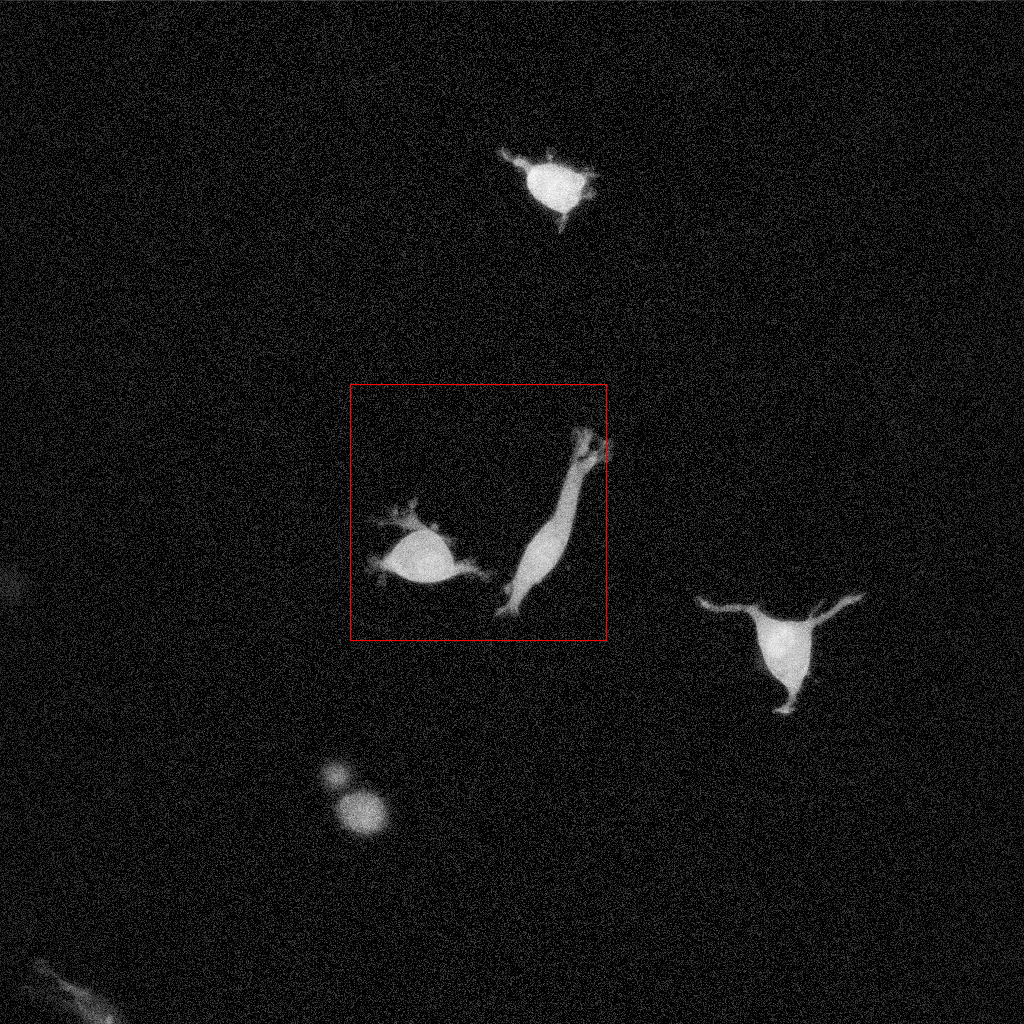
\includegraphics[width=.2\textwidth]{img/0-first-full.png}
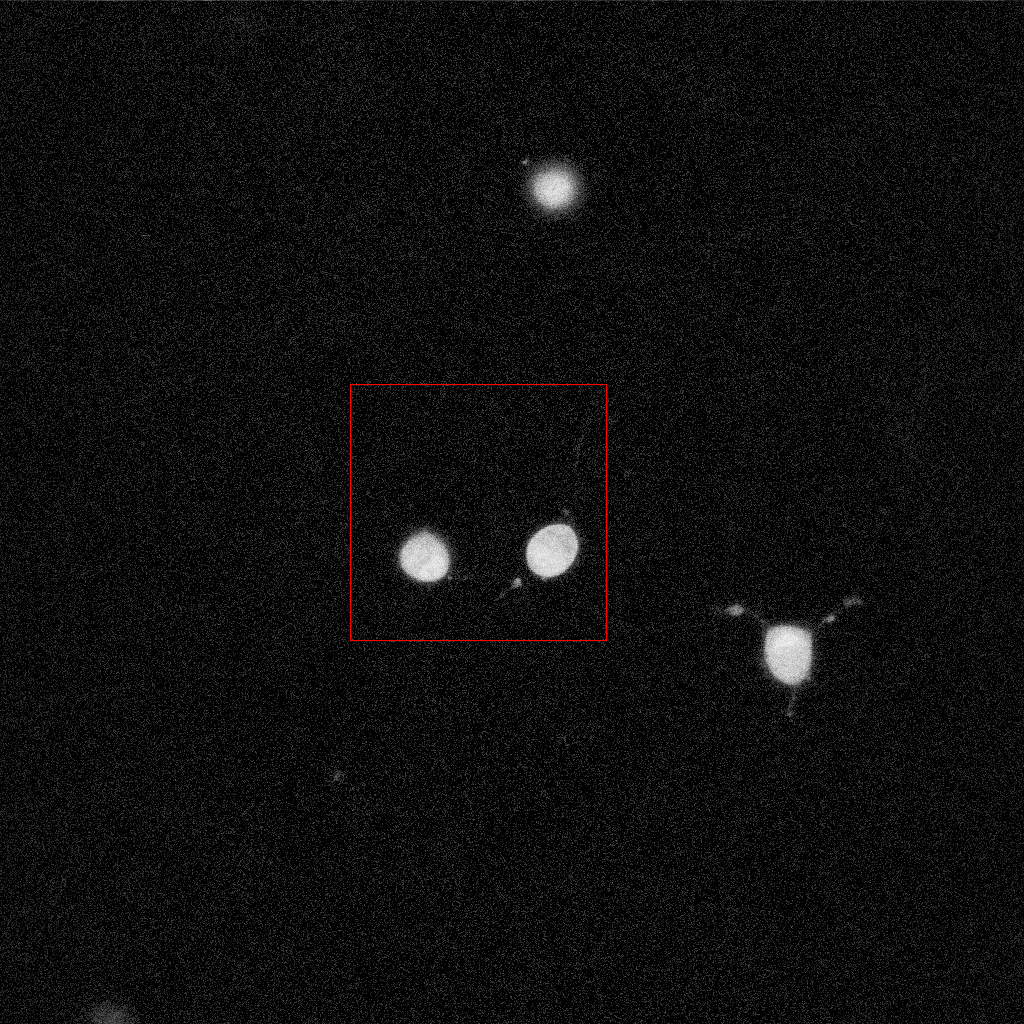
\includegraphics[width=.2\textwidth]{img/0-last-full.png}
\caption{\label{fig:0-full}MIP of first and last z-stacks from an experiment with the region of interest outlined in red}
\end{figure}

\section*{conclusions}
The plotted numerical data in figure~\ref{fig:resultPlots} appears to show that area and eccentricity both decrease as time progresses. Analyis of data from further experiments might allow one to model size and eccentricity of cells as they release a substrate. One could use this model to predict size and area of fibroblasts when trypsinized.

To improve the results of this data, I would take a taller z-stack, take images more frequently, and adjust the brightening factor to increase smoothness in images. Using taller z-stacks should better capture entire cells as they move away from the surface of the collagen. More frequent images would increase data. Adjusting the brightening factor could reduce noise which is amplified when using the im2bw funtion.

%Acquiring images more frequently would likely increase smoothness of the plotted data. Seemingly, data collected would be more accurate using a taller z-stack. Taller z-stacks give more data points to analyze, possibly removing fluctuations in this data set.
%
%Accuracy of the numerical data could be improved by minimizing the noise introduced when transforming the greyscale images into binary images. This noise could be reduced by adjusting the brightening factor and adjusting the threshold used to create the binary images. For this, maximize a function that increases appropriately with area while decreasing appropriately with "roughness."

%The data suggests that the area and eccentricity both decrease as time progresses. For this reason, the analysis of the data seems to confirm that a flattened out cell shrinks back into a ball. Still, the methods suggested to improve data collection and analysis could be used to model fibroblast-morphology during trypsinization.


\clearpage
\onecolumngrid
\begin{center}
\begin{figure}[h!]
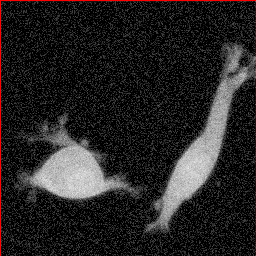
\includegraphics[width=.3\textwidth]{img/0-first.png}
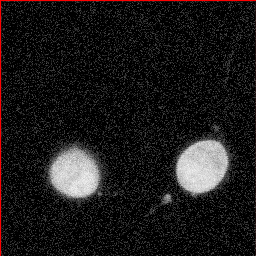
\includegraphics[width=.3\textwidth]{img/0-last.png}\\
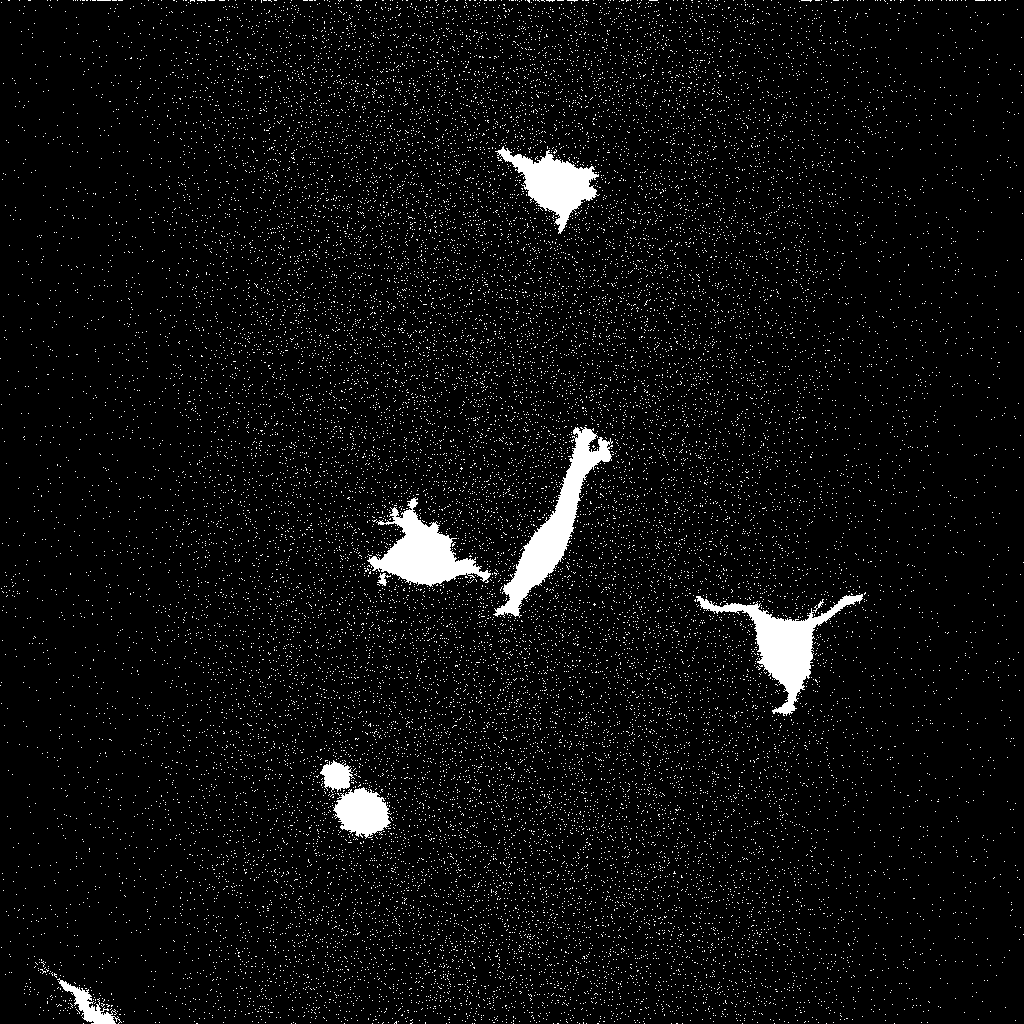
\includegraphics[width=.3\textwidth]{img/1-first.png}
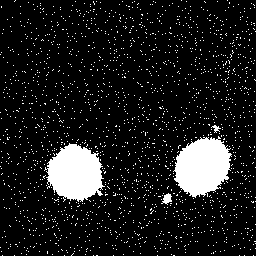
\includegraphics[width=.3\textwidth]{img/1-last.png}\\
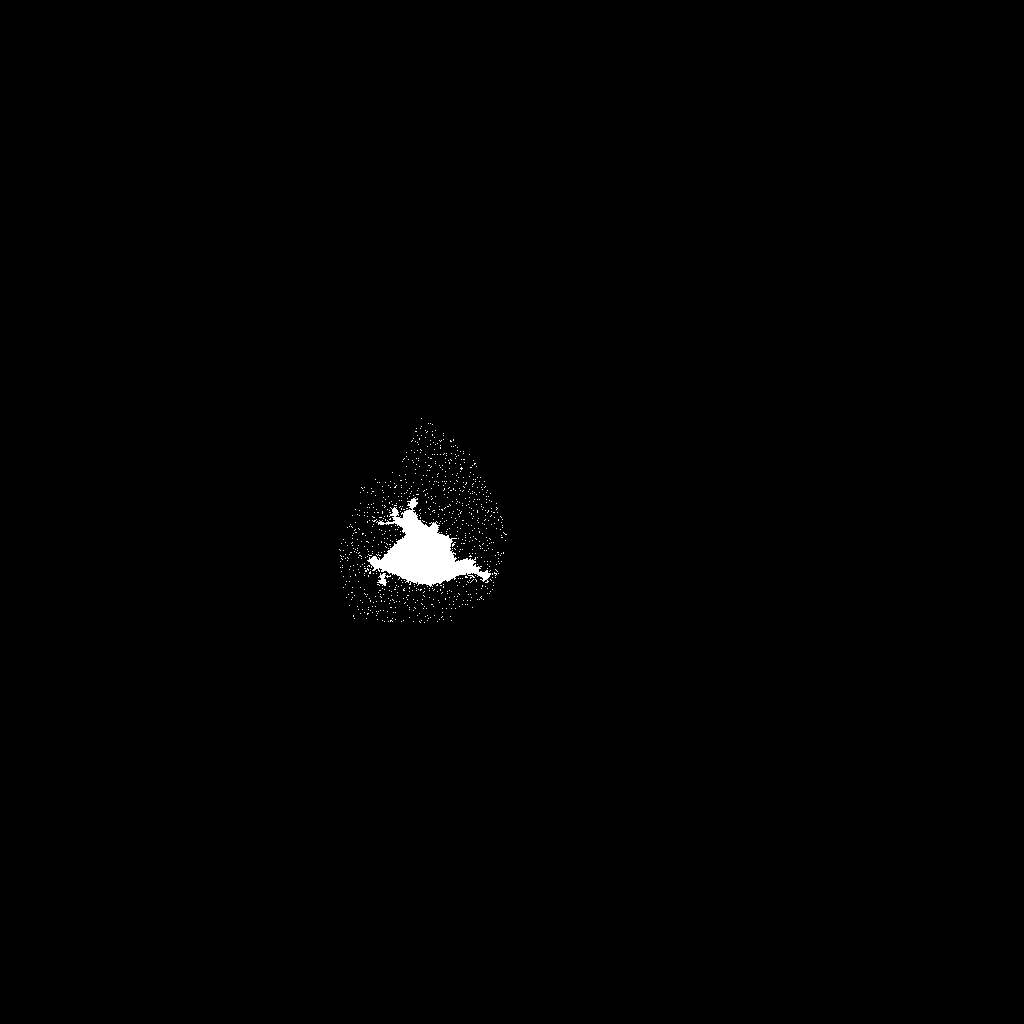
\includegraphics[width=.3\textwidth]{img/2-first.png}
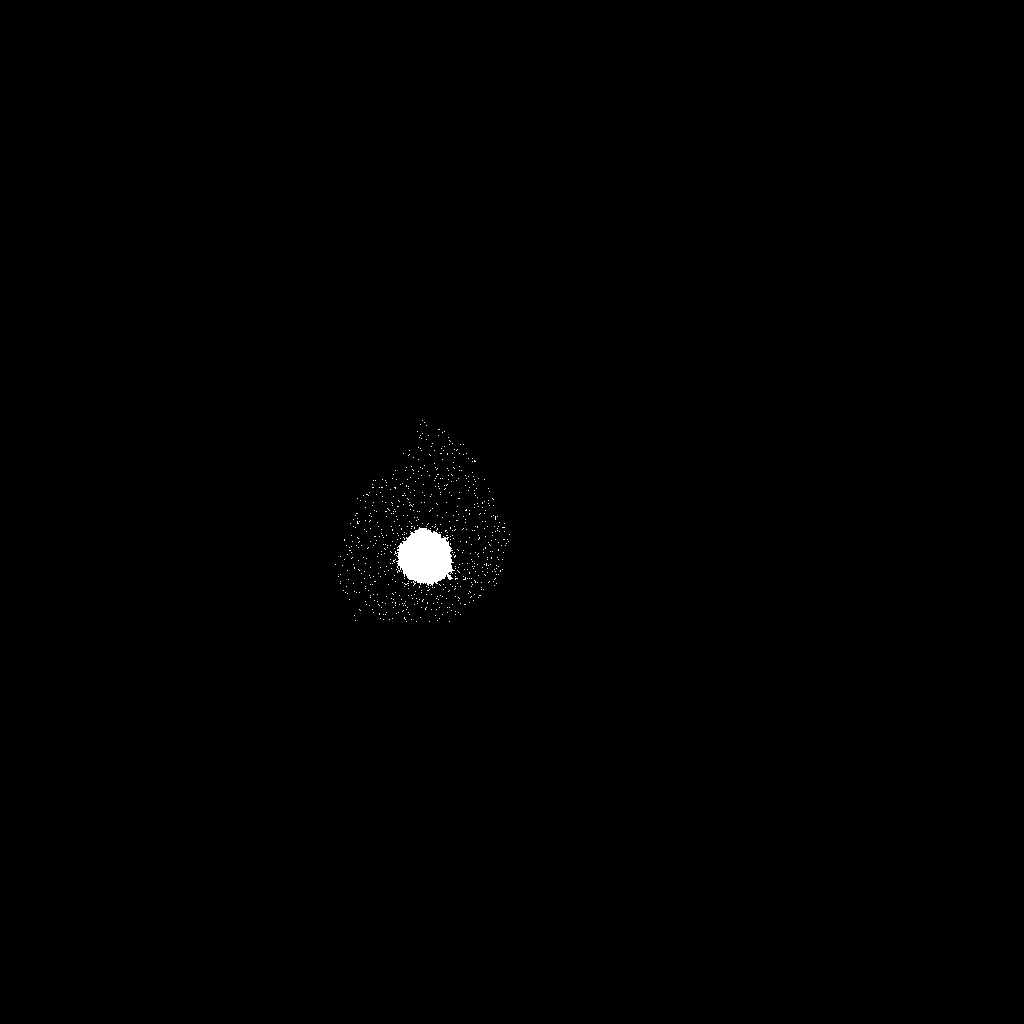
\includegraphics[width=.3\textwidth]{img/2-last.png}\\
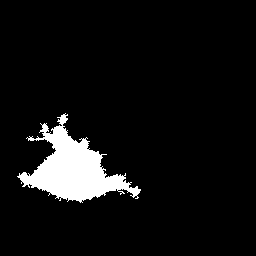
\includegraphics[width=.3\textwidth]{img/3-first.png}

\includegraphics[width=.3\textwidth]{img/3-last.png}\\
\caption{\label{fig:0123}Region of interest from FIG.~\ref{fig:0-full} at several stages throughout image processing; from top to bottom, the rows show the original images, the result of 'binarization', the result of masking, and the segmented cell from the images.}
\end{figure}

%\section*{results}
%Figure \ref{fig:resultPlots} plots the data from the experiment as labeled. Table \ref{tab:resultTable} presents numerical data from the experiment's images.

\begin{figure}
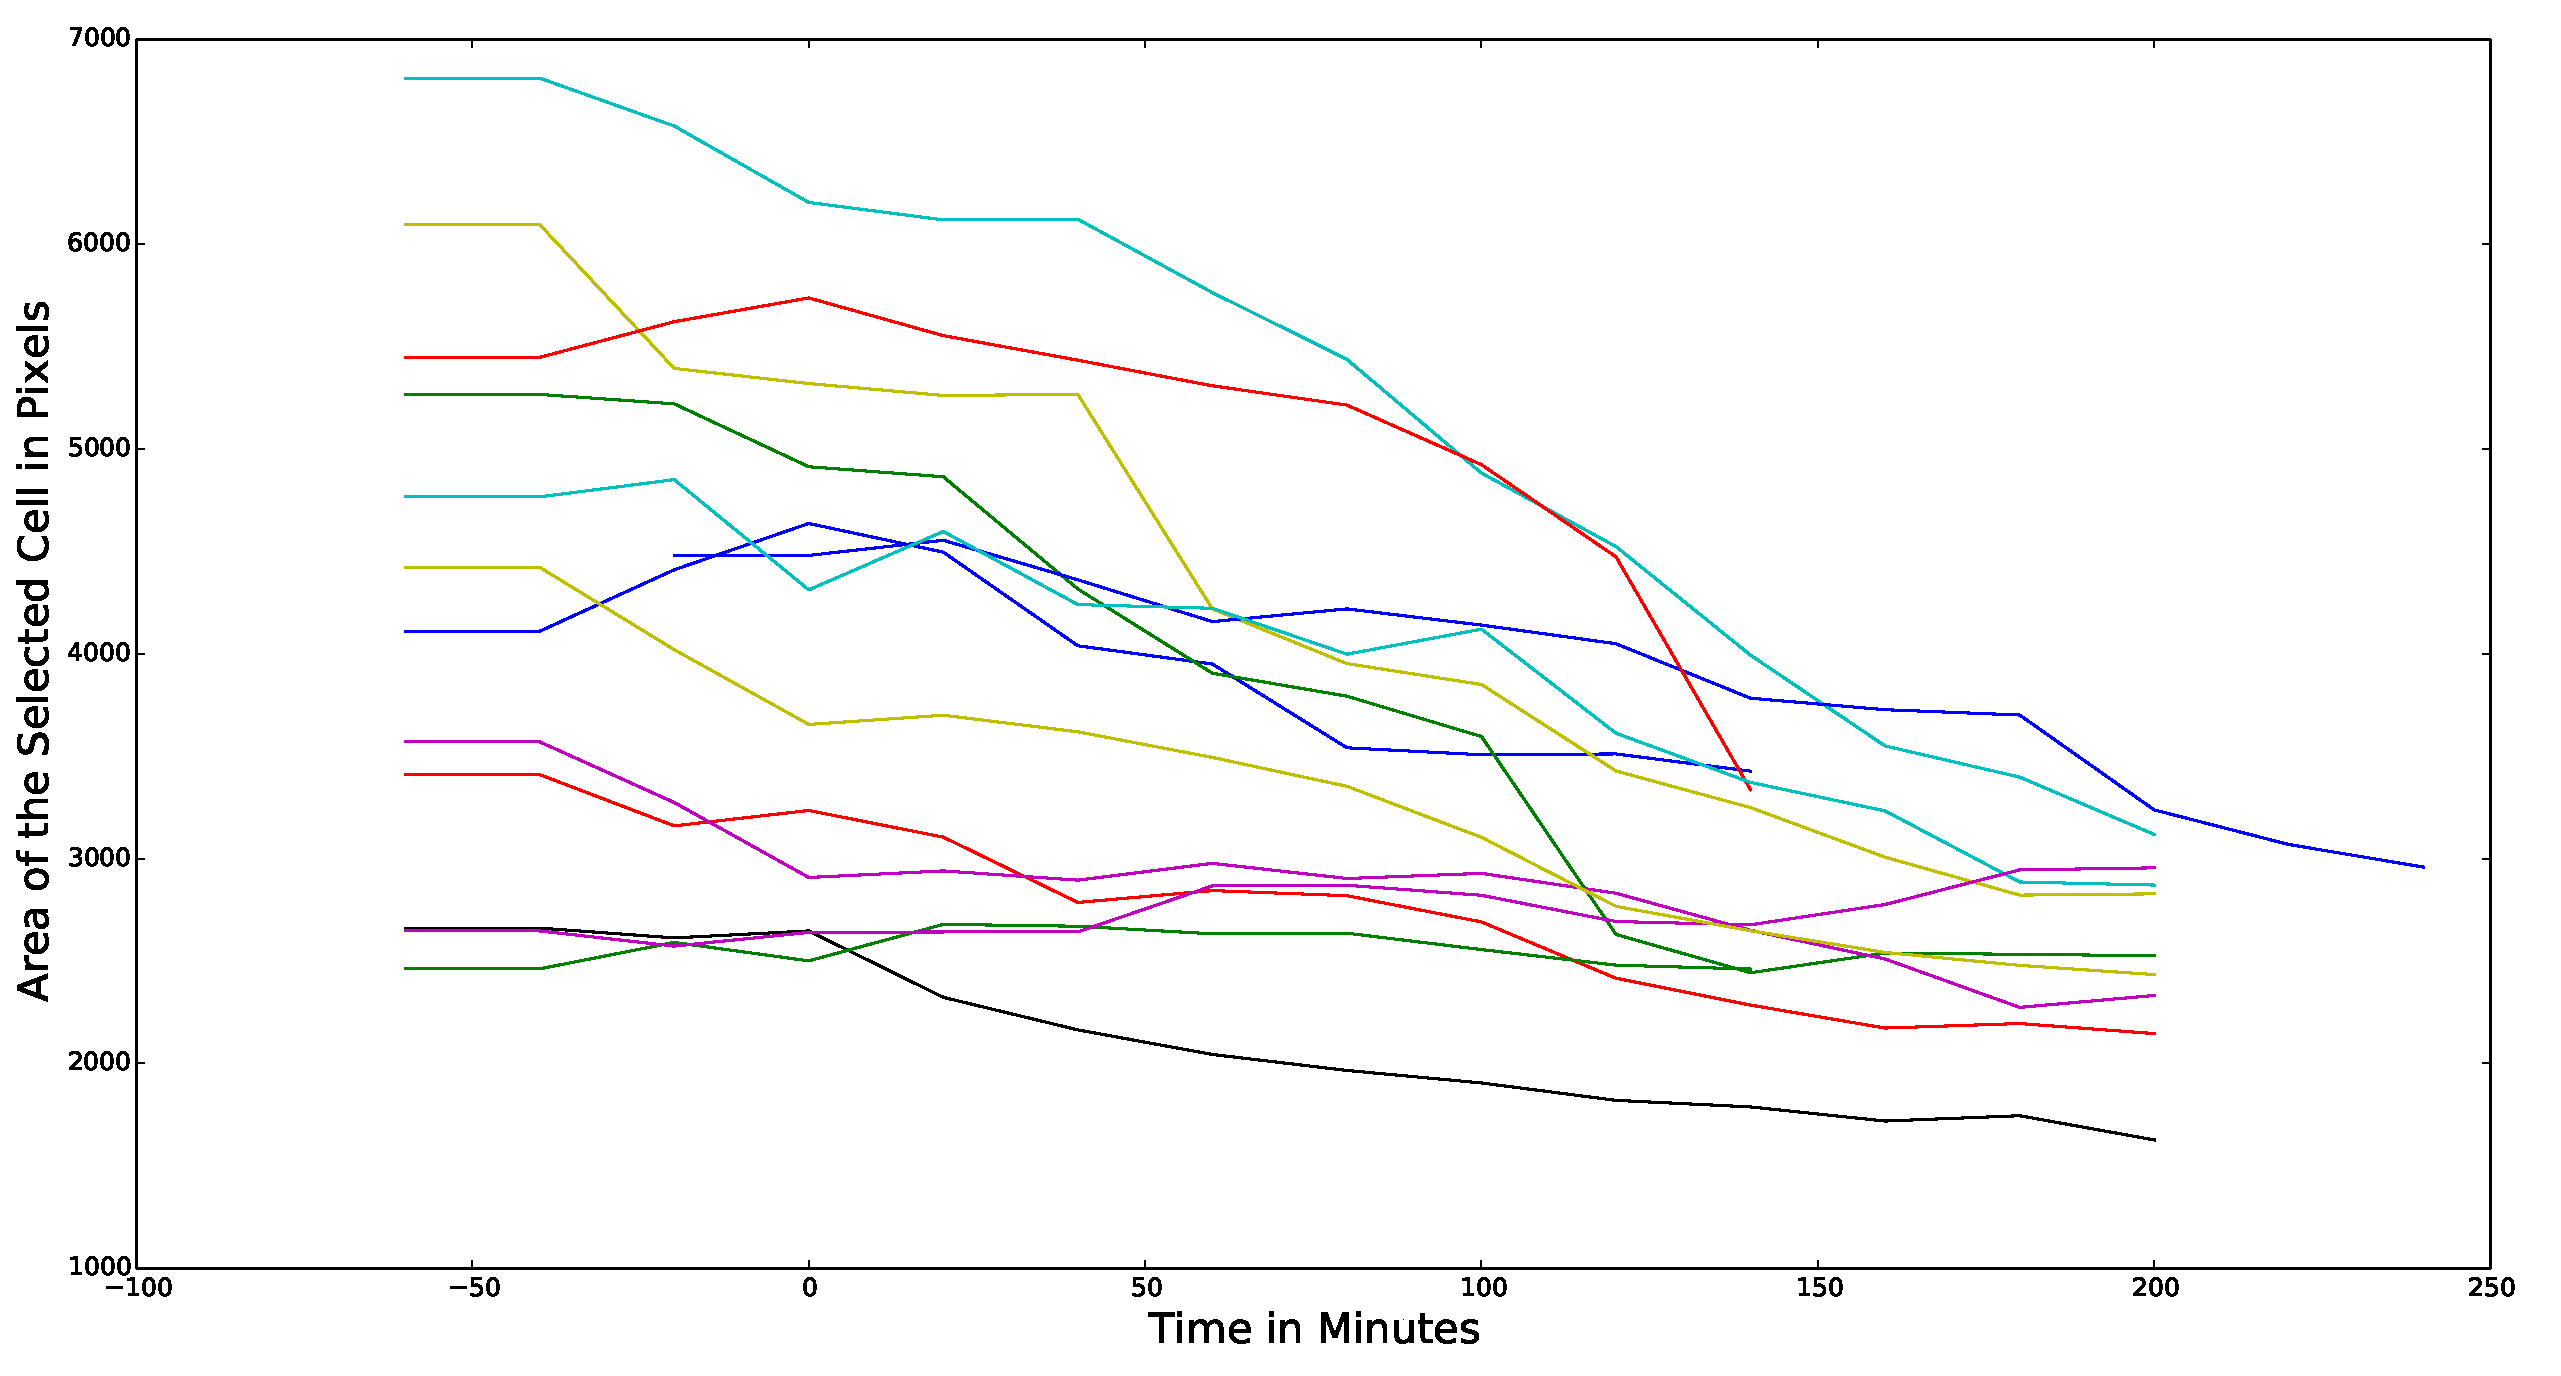
\includegraphics[width=.95\textwidth]{img/mplAreaVsTime.pdf}
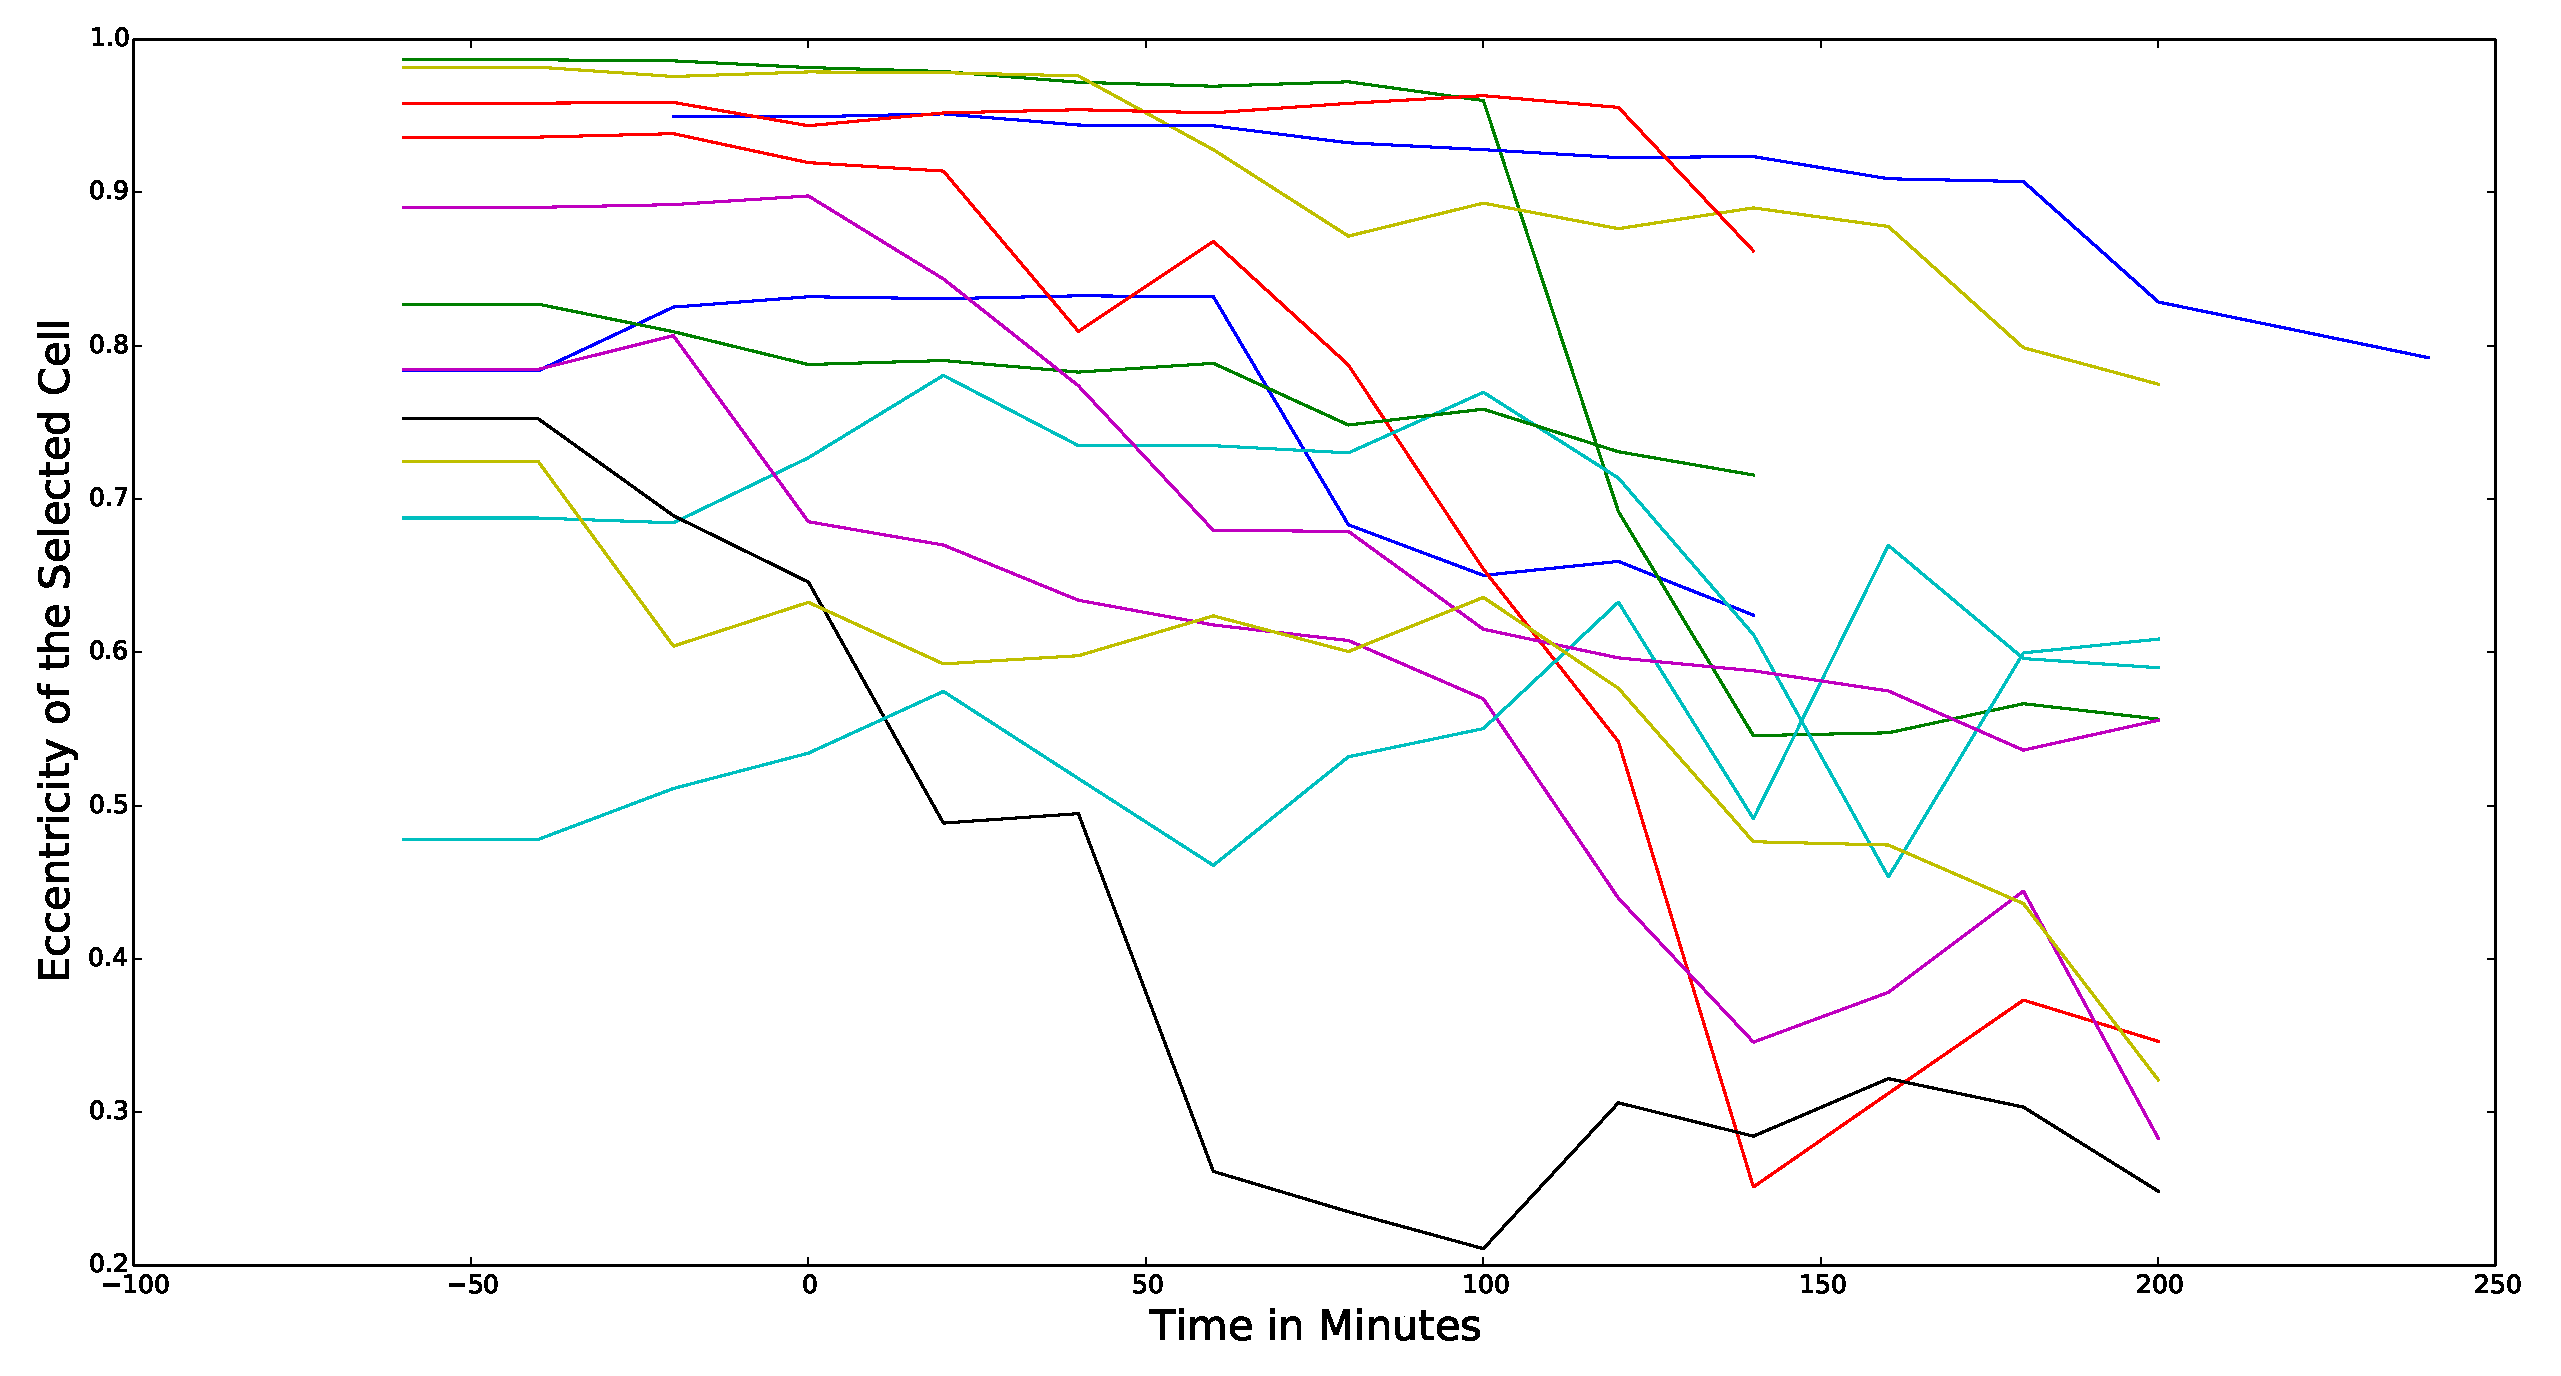
\includegraphics[width=.95\textwidth]{img/mplEccentricityVsTime.pdf}
\caption{\label{fig:resultPlots}Plots of experimental data: Area Vs. Time and Eccentricity Vs. Time}
\end{figure}
\end{center}

%\section*{acknowlegements}

%\section*{References}

%\clearpage\newpage
%\section*{Appendices}
%\subsection*{Appendix A: Experiment Protocol}
%The protocol for creating three collagen-samples of concentration 1.5 and gelled at 21$^{\circ}$C is as follows:
%\begin{enumerate}
%	\item Create the collagen-solution.
%	\begin{enumerate}
%		\item Total volume to be made is V = (90$\mu$L per sample)(3 samples)(150\%) = 405$\mu$L.
%		\item Combine 40.5$\mu$L 10X PBS, 14.2$\mu$L NaOH, and 276.3$\mu$L growth-medium.
%		\item Shake this solution at 400rpm for 20 seconds.
%		\item Store at 6$^{\circ}$C for 10 minutes.
%		\item Add 71$\mu$L collagen homogeneously.
%		\item Stir collagen into solution with a 100$\mu$L pipette tip.
%		\item Pipette 90$\mu$L collagen-solution into each of the 3 samples a, b, and c.
%		\end{enumerate}
%	\item Wrap each sample in film and let gelate at 21$^{\circ}$C for two hours.
%	\item Place growth-medium on all samples and place cells on sample a.
%	\item Place cells on sample b four hours later.
%	\item Place cells on sample c four hours later.
%	\item Using confocal fluorescence microscopy, capture a 10$\mu$m tall z-stack of images of fibers and cells, separately, every 20 minutes for four hours.
%	\begin{enumerate}
%		\item After the first z-stack, replace the growth-medium on the sample with 1X PBS.
%		\item After the second z-stack, replace the PBS with fresh PBS.
%		\item After the third z-stack, replace the PBS with 1X TrypLe\texttrademark\hspace{.1em} Select.
%	\end{enumerate}
%		\item When sample a is finished imaging, image sample b in the same way as sample a was imaged.
%		\item When sample b is finished imaging, image sample c in the same way as sample a was imaged.
%\end{enumerate}
 
\onecolumngrid
\clearpage
\appendix*
\section{Code (to be used and distributed freely)}
\lstinputlisting[ language=Matlab,
                  caption=segmenter.m,
                  label=segmenter ]
                {code/matlab/segmenter.m}

\clearpage
\lstinputlisting[ language=Matlab,
                  caption=stackreader.m,
                  label=stackreader
                ]{code/matlab/stackreader.m}

\lstinputlisting[ language=Matlab,
                  caption=stackwriter.m,
                  label=stackwriter
                ]{code/matlab/stackwriter.m}

\lstinputlisting[ language=Matlab,
                  caption=maskmaker.m,
                  label=maskmaker
                ]{code/matlab/maskmaker.m}

\lstinputlisting[ language=Matlab,
                  caption=stackmasker.m,
                  label=stackmasker
                ]{code/matlab/stackmasker.m}

\lstinputlisting[ language=Matlab,
                  caption=ExtractNLargestBlobs.m,
                  label=ExtractNLargestBlobs
                ]{code/matlab/ExtractNLargestBlobs.m}

\clearpage
\lstinputlisting[ language=Matlab,
                  caption=tinker.m,
                  label=tinker
                ]{code/matlab/tinker.m}

\lstinputlisting[ language=Matlab,
                  caption=regionPropsScript.m,
                  label=regionPropsScript
                ]{code/matlab/regionPropsScript.m}

%\section*{TODO:}
%\begin{enumerate}
%\item insert results with plots
%\item write a conclusion
%\item write acknowledgements
%\item discuss binarizing giving noise b/c thresholding not optimal
%\item Sometimes a cell appears to getting smaller then randomly appears larger then returns to its shrinking behavior, and at the area/eccentricity it would have been if it never got wacky. In results, discuss how using a taller z-stack centered about the gel-surface might have "settled the data's spuratic behavior." Taller z-stack might have better observed the z-directed movement of the cells, which might be causing some of the sudden-seeming changes and reversals of the direction of area/eccentricity changes... 

%\end{enumerate}
\end{document}
